
\subsection{Transferencia del circuito}

Aqu\'i se compara la funci\'on transferencia del circuito te\'orica, 
medida y simulada mediante el m\'etodo de Montecarlo. Para la medici\'on se emple\'o el bodeador realizado para este trabajo. La simulaci\'on se llev\'o a cabo considerando tolerancias de $1\%$ para las resistencias ya que las empleadas fueron SMD y $10\%$ para los capacitores hole through. Adem\'as, se aclara que la simulaci\'on fue realizada incluyendo las impedancias equivalentes de $10M\Omega // 12pF$ aportadas por las puntas del osciloscopio que se usaron para tomar las mediciones.

\begin{figure}[H] %!ht
	\centering
	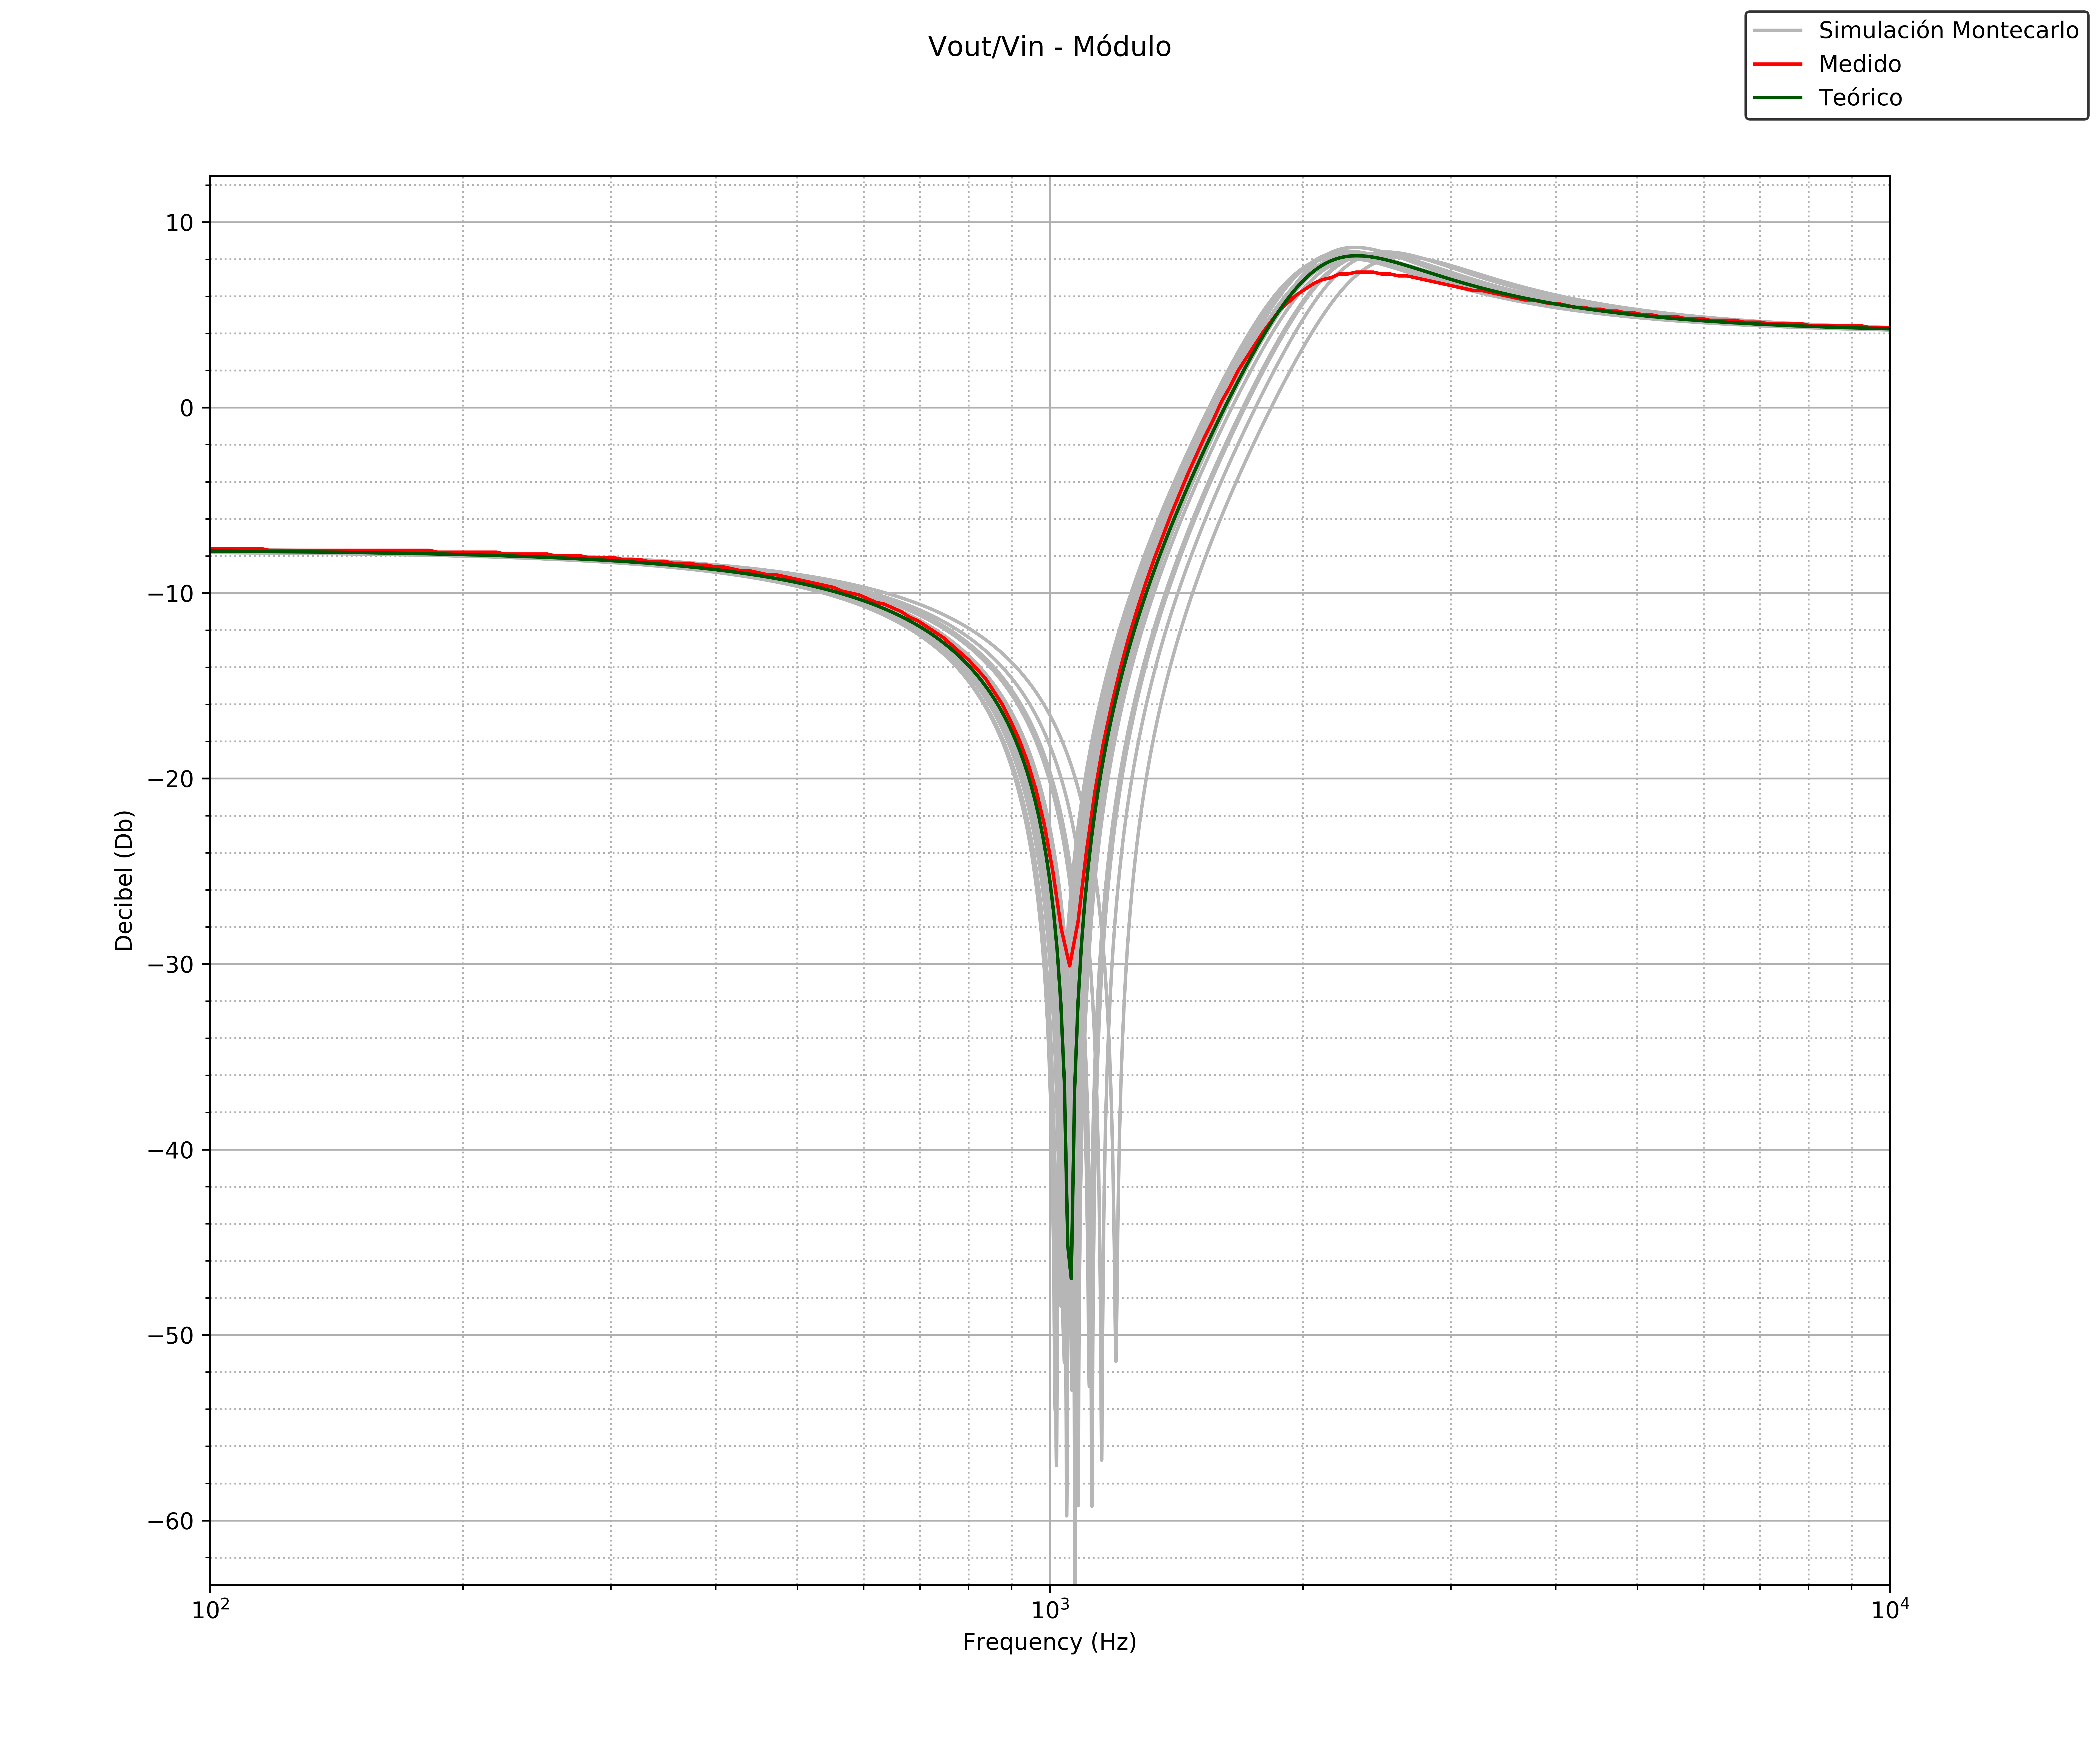
\includegraphics[width=10cm,height=10cm,keepaspectratio]{../EJ1/00GRAFICOS/vovi.png}
	\caption{M\'odulo de la transferencia del circuito.}
	\label{vovi_mod}
\end{figure}

\begin{figure}[H] %!ht
	\centering
	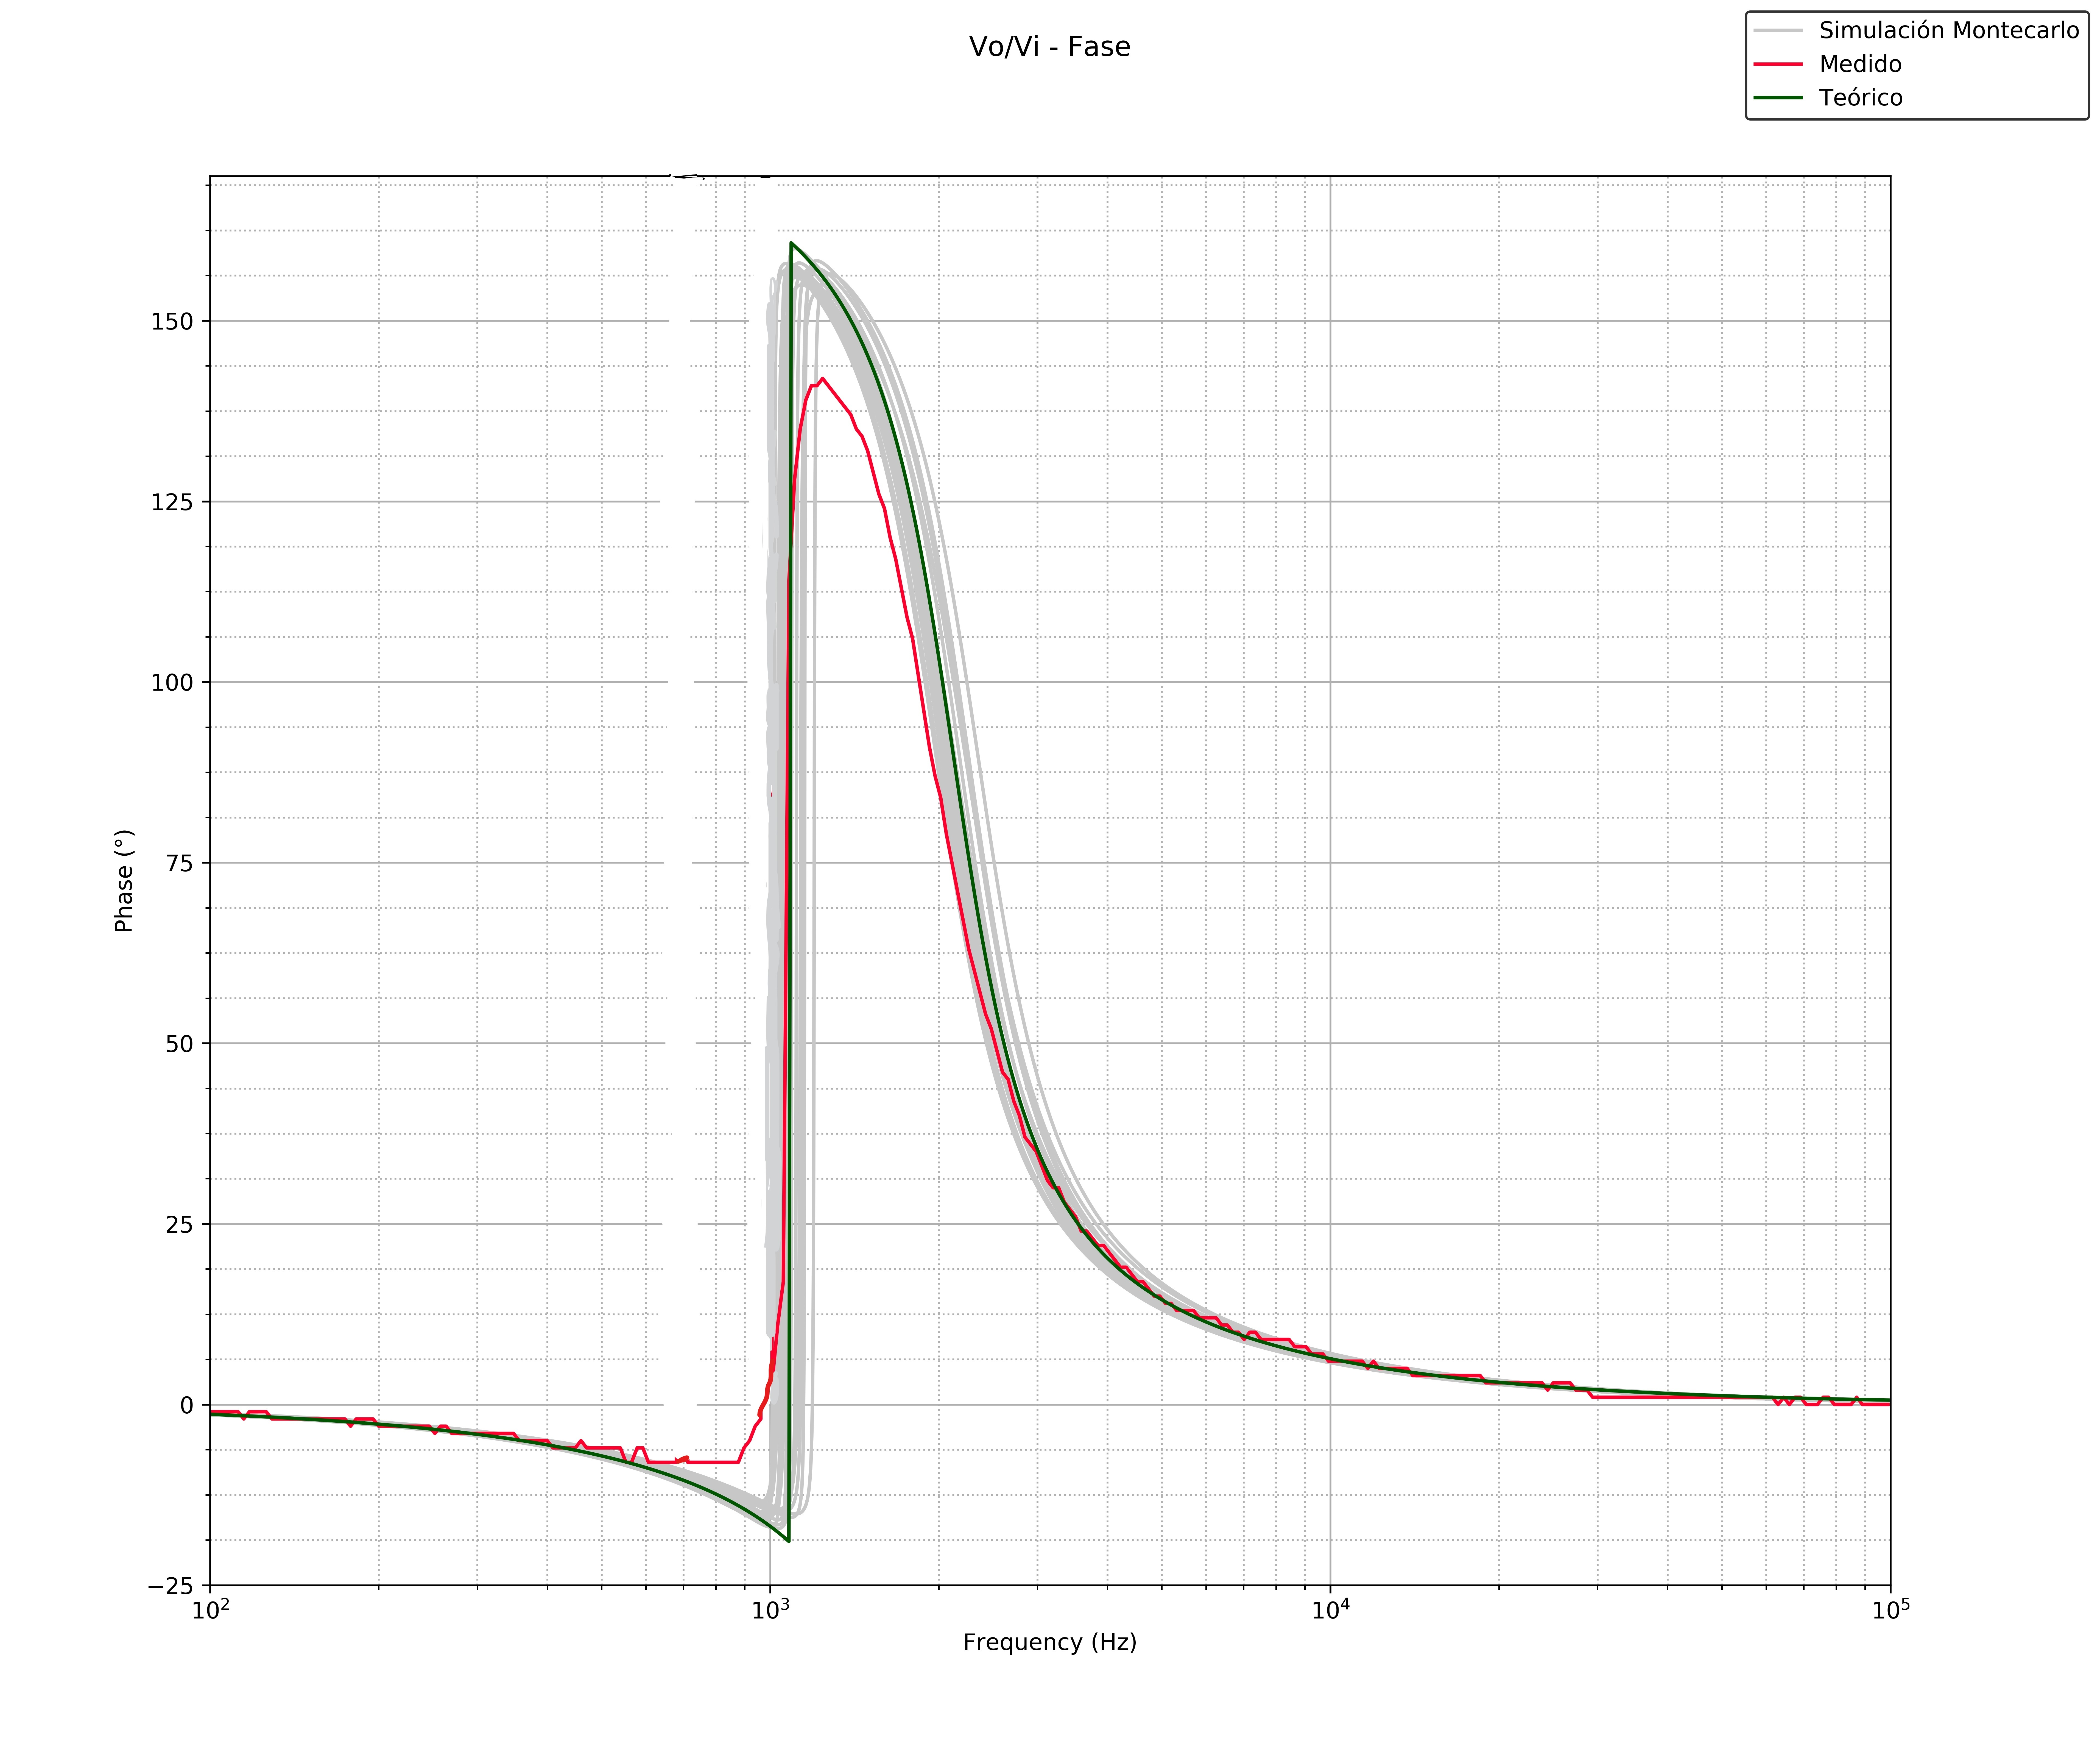
\includegraphics[width=10cm,height=10cm,keepaspectratio]{../EJ1/00GRAFICOS/vovifase.jpg}
	\caption{Fase de la transferencia del circuito.}
	\label{vovi_fase}
\end{figure}

El gr\'afico del m\'odulo de la funci\'on transferencia, figura \ref{vovi_mod}, permite ver que los Q de la medici\'on fueron menores que aquellos de los c\'alculos te\'oricos. Si bien el Q del polo presenta una peque\~na respecto a la especificada te\'oricamente en el dise\~no del circuito, el Q del cero presenta un cambio notable. Te\'oricamente el mismo deb\'a ser infinito, pero en la implementaci\'on eso no ocurre. Sin embargo, la atenuaci\'on no deja de ser considerable.

